\textbf{Seats}
\begin{enumerate}
    \item 10 mins: Intro slides \par
    \item 15 mins: Finish Example 4.6.3 \par
    \textbf{Check piazza}
    \item 25 mins: Finish Example 4.6.4 \par
    \textbf{Check piazza}
    \textbf{Motivation}
    \item 40 mins: Finish Example 5.1.1 \par
    \textbf{Check piazza}
    \item 50 mins: Finish Example 5.1.2 \par
\end{enumerate}
\textbf{Seats}

\newcommand{\vect}[1]{\underline{\mathbf{#1}}}

\vspace{5mm} 

\textbf{Example 4.6.3} \par

Can just do this by saying $\vect{a}\times\vect{b}$ is perpendicular to $\vect{a}$ so $\vect{a}\cdot(\vect{a}\times\vect{b}) = 0$.

In component form
\begin{align*}
\begin{vmatrix}
    a_x & a_y & a_z\\
    a_x & a_y & a_z \\
    b_x & b_y & b_z
\end{vmatrix} &= a_x(a_y b_z - a_z b_y) + a_y(a_z b_x - a_x b_z) + a_z (a_x b_y - a_y b_x) \\
&= a_x a_y b_z - a_x b_y a_z + b_x a_y a_z - a_x a_y b_z + a_x b_y a_z - b_x a_y a_z\\
&= 0
\end{align*}
The first and fourth, second and fifth, and third and sixth terms cancel.

\textbf{Example 4.6.4} \par

First, calculate $\vect{b} \times \vect{c}$, which we will call $\vect{v}$,
\begin{align*}
    \vect{v} = \vect{b} \times \vect{c} = \begin{vmatrix}
        \vect{i} & \vect{j} & \vect{k} \\
        -1 & 0 & 5 \\
        6 & -1 & 0
    \end{vmatrix} &= (0+5)\vect{i} + (30-0)\vect{j} + (1-0)\vect{k}\\
    &= 5\vect{i} + 30\vect{j} + \vect{k} \,.
\end{align*}
Now do $\vect{a} \times \vect{v}$,
\begin{align*}
    \vect{a} \times (\vect{b} \times \vect{c}) = \begin{vmatrix}
        \vect{i} & \vect{j} & \vect{k} \\
        2 & 2 & -1 \\
        5 & 30 & 1
    \end{vmatrix} &= (2+30)\vect{i} + (-5-2)\vect{j} + (60-10)\vect{k}\\
    &= 32\vect{i} - 7\vect{j} + 50\vect{k} \,.
\end{align*}
Now consider the other formula
\begin{align*}
    \vect{a}\cdot\vect{c} &= (2 \times 6) + (2\times(-1)) = 10\\
    \vect{a}\cdot\vect{b} &= (2\times(-1))+((-1)\times5)=-7 \, .
\end{align*}
Therefore
\begin{align*}
    (\vect{a}\cdot\vect{c})\vect{b} - (\vect{a}\cdot\vect{b})\vect{c} = 10\vect{b} + 7\vect{c} &= \begin{pmatrix}
        -10 \\ 0 \\ 50
    \end{pmatrix} + \begin{pmatrix}
        42 \\ -7 \\ 0
    \end{pmatrix} \\
    &= 32 \vect{i} - 7 \vect{j} + 50 \vect{k}
\end{align*}

\textbf{Example 5.1.1} \par

\begin{align*}
    z^2 = -1 \quad \rightarrow \quad z &= \pm i\\
    z^2 = -16 \quad \rightarrow \quad z &= \pm 4i\\
    z^2 = -28 \quad \rightarrow \quad z &= \pm 2\sqrt{7} i
\end{align*}

\textbf{Example 5.1.2} \par

\begin{table}[h!]
    \centering
    \begin{tabular}{|c|c|c|c|}
            & Re$(z)$ & Im$(z)$ & $\bar{z}$ \\ \hline
     $z_1 = 2+5i$  & 2 & 5 & 2-5i\\
     $z_2 = -7-2i$ & -7 & -2 & -7+2i\\
    \end{tabular}
    \caption{Real and imaginary parts and conjugates.}
    \label{tab:ex_512}
\end{table}

\begin{figure}[h!]
    \centering
    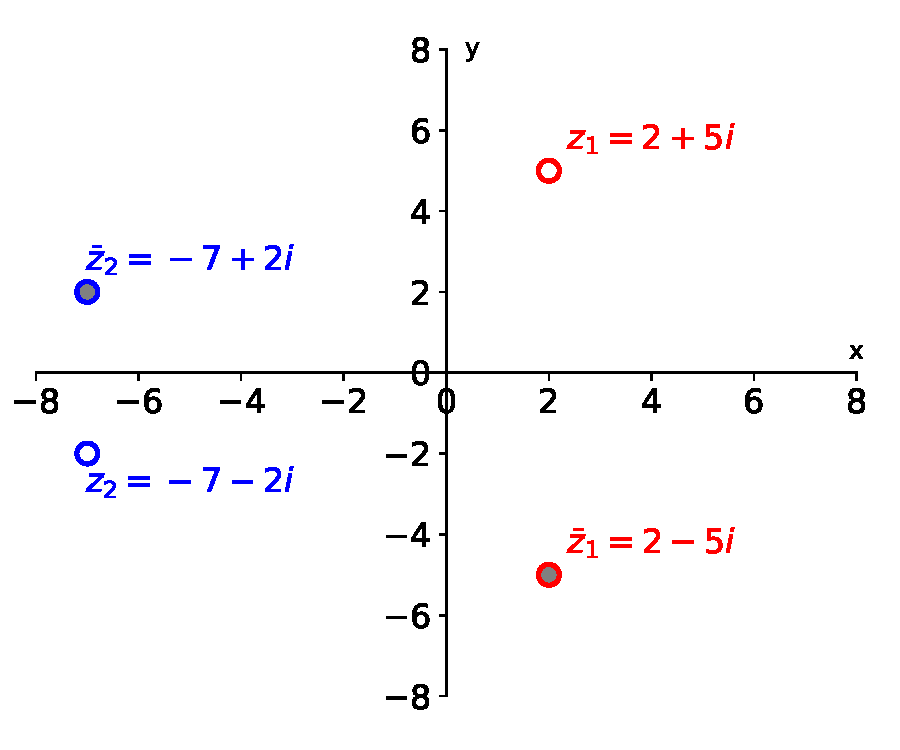
\includegraphics[width=0.5\linewidth]{Figures/example_512.pdf}
    \caption{Argand diagram}
    \label{fig:ex_512}
\end{figure}